\newpage
\section{La Fonction Delta de Dirac}

\subsection{Introduction et Définition}

Après avoir étudié des distributions continues classiques comme la loi normale et log-normale, nous abordons un objet mathématique singulier : la \textit{fonction delta de Dirac}, notée $\delta(x)$. Bien qu'elle ne soit pas une fonction au sens classique, elle est fondamentale en probabilités.

\begin{definitionbox}[Fonction Delta de Dirac]
La \textbf{fonction delta de Dirac} $\delta(x)$ est une \textit{distribution} (ou fonction généralisée) caractérisée par deux propriétés :
\begin{enumerate}
    \item $\delta(x) = 0$ pour tout $x \neq 0$,
    \item $\int_{-\infty}^{+\infty} \delta(x) \, dx = 1$.
\end{enumerate}

Intuitivement, $\delta(x)$ représente une « masse ponctuelle » d'intensité infinie localisée en $x = 0$, mais d'aire totale égale à 1.
\end{definitionbox}

\begin{remarquebox}[Paradoxe Apparent]
Ces deux propriétés semblent contradictoires : comment une fonction nulle partout sauf en un point peut-elle avoir une intégrale égale à 1 ?

La résolution du paradoxe vient du fait que $\delta(x)$ n'est \textbf{pas une fonction ordinaire}, mais une \textit{distribution} au sens de Laurent Schwartz. Elle ne prend pas de « valeur » en un point, mais agit sur d'autres fonctions via l'intégration. On dit que $\delta$ est une \textbf{mesure de Dirac} concentrée en 0.
\end{remarquebox}

\subsection{Intuition : De la Masse Diffuse à la Masse Ponctuelle}

La delta de Dirac peut être comprise comme la limite d'une suite de fonctions de plus en plus « piquées ».

\begin{intuitionbox}[Approximation par des Fonctions Régulières]
\textbf{1. Idée de Base} :

Imaginons une distribution de masse sur la droite réelle. Au lieu d'être étalée, nous voulons concentrer toute la masse en un seul point (l'origine), tout en préservant la masse totale.

\textbf{2. Construction par Limite (Gaussiennes)} :

Considérons la famille de gaussiennes centrées en 0 :
$$ \delta_\epsilon(x) = \frac{1}{\epsilon\sqrt{2\pi}} \exp\left(-\frac{x^2}{2\epsilon^2}\right) $$

\begin{itemize}
    \item Pour tout $\epsilon > 0$, $\delta_\epsilon(x)$ est une densité de probabilité normale $\mathcal{N}(0, \epsilon^2)$.
    \item $\int_{-\infty}^{+\infty} \delta_\epsilon(x) \, dx = 1$ (aire sous la courbe = 1).
    \item Quand $\epsilon \to 0$ :
    \begin{itemize}
        \item La hauteur du pic augmente : $\delta_\epsilon(0) = \frac{1}{\epsilon\sqrt{2\pi}} \to +\infty$.
        \item La largeur diminue : la variance $\epsilon^2 \to 0$.
        \item Pour tout $x \neq 0$, $\delta_\epsilon(x) \to 0$ (la queue s'aplatit).
        \item L'aire totale reste 1.
    \end{itemize}
\end{itemize}

On écrit symboliquement :
$$ \delta(x) = \lim_{\epsilon \to 0} \delta_\epsilon(x) $$

\textbf{3. Autres Approximations Possibles} :

On peut obtenir $\delta(x)$ comme limite de nombreuses familles de fonctions :
\begin{itemize}
    \item \textbf{Rectangles} : $\delta_\epsilon(x) = \begin{cases} \frac{1}{2\epsilon} & \text{si } |x| < \epsilon \\ 0 & \text{sinon} \end{cases}$
    \item \textbf{Lorentziennes} : $\delta_\epsilon(x) = \frac{1}{\pi} \cdot \frac{\epsilon}{\epsilon^2 + x^2}$
    \item \textbf{Sinus cardinal} : $\delta_\epsilon(x) = \frac{1}{\pi x} \sin\left(\frac{x}{\epsilon}\right)$ (avec régularisation)
\end{itemize}

Toutes ces fonctions « tendent » vers $\delta(x)$ au sens des distributions.

\tcblower
\centering
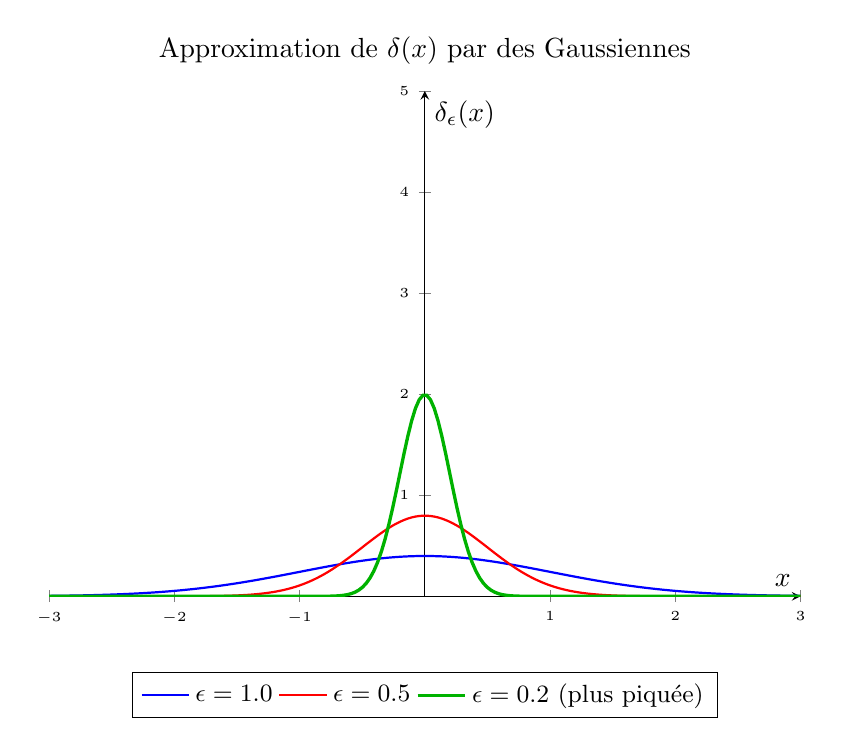
\begin{tikzpicture}
    \begin{axis}[
        title={Approximation de $\delta(x)$ par des Gaussiennes},
        xlabel={$x$},
        ylabel={$\delta_\epsilon(x)$},
        axis lines=middle,
        no markers,
        samples=200,
        domain=-3:3,
        ymin=0, ymax=5,
        height=8cm,
        width=\linewidth-1cm,
        tick label style={font=\tiny},
        legend style={at={(0.5,-0.15)}, anchor=north, font=\small},
        legend columns=3
    ]
    % Gaussienne epsilon = 1
    \addplot [blue, thick] {1/(1*sqrt(2*pi))*exp(-(x^2)/(2*1^2))};
    \addlegendentry{$\epsilon=1.0$};
    % Gaussienne epsilon = 0.5
    \addplot [red, thick] {1/(0.5*sqrt(2*pi))*exp(-(x^2)/(2*0.5^2))};
    \addlegendentry{$\epsilon=0.5$};
    % Gaussienne epsilon = 0.2
    \addplot [green!70!black, very thick] {1/(0.2*sqrt(2*pi))*exp(-(x^2)/(2*0.2^2))};
    \addlegendentry{$\epsilon=0.2$ (plus piquée)};
    \end{axis}
\end{tikzpicture}
\par\small\textit{Quand $\epsilon \to 0$, la hauteur $\to \infty$, la largeur $\to 0$, mais l'aire reste $= 1$.}
\end{intuitionbox}

\subsection{Propriété Fondamentale : La Propriété de Filtrage}

La définition vraiment opérationnelle de $\delta(x)$ repose sur son action sur les fonctions continues.

\begin{theorembox}[Propriété de Filtrage (Sifting Property)]
Pour toute fonction $f$ continue en $x = 0$ :
$$ \int_{-\infty}^{+\infty} f(x) \, \delta(x) \, dx = f(0) $$

Plus généralement, $\delta$ décalé en $a$ filtre la valeur en $a$ :
$$ \int_{-\infty}^{+\infty} f(x) \, \delta(x - a) \, dx = f(a) $$
\end{theorembox}

\begin{proofbox}[Justification Intuitive]
Utilisons l'approximation gaussienne $\delta_\epsilon(x) = \frac{1}{\epsilon\sqrt{2\pi}} e^{-x^2/(2\epsilon^2)}$.

On a :
$$ \int_{-\infty}^{+\infty} f(x) \, \delta_\epsilon(x) \, dx = \mathbb{E}[f(X)] \quad \text{où } X \sim \mathcal{N}(0, \epsilon^2) $$

Quand $\epsilon \to 0$, la loi de $X$ se concentre entièrement en $x = 0$. Donc :
$$ \lim_{\epsilon \to 0} \mathbb{E}[f(X)] = f(0) \quad \text{(par continuité de } f \text{)} $$

Pour $\delta(x - a)$, le raisonnement est identique en centrant la gaussienne en $a$.
\end{proofbox}

\begin{remarquebox}[Interprétation Probabiliste]
En théorie des probabilités, $\delta(x - a)$ est la « densité » (au sens des distributions) d'une variable aléatoire \textbf{dégénérée} qui prend la valeur $a$ avec probabilité 1.

Si $X = a$ presque sûrement, alors pour toute fonction mesurable $f$ :
$$ \mathbb{E}[f(X)] = f(a) = \int_{-\infty}^{+\infty} f(x) \, \delta(x - a) \, dx $$

Ainsi, $\delta(x - a)$ généralise la notion de densité de probabilité aux masses ponctuelles.
\end{remarquebox}

\begin{examplebox}[Loi de Durée de Vie d’un Dispositif — Mélange Discret/Continu]
\textbf{Contexte} : Une entreprise produit des dispositifs dont la durée de vie $X$ (en années) n’est pas toujours continue. En effet, environ 2\% des dispositifs sont défectueux dès le départ : leur durée de vie est donc exactement $0$ an. Pour les 98\% restants, la durée de vie suit une loi exponentielle de paramètre $\lambda = 2$ an$^{-1}$.

\textbf{Objectif} : Déterminer la \textbf{densité généralisée} de $X$, qui mélange une masse de Dirac en 0 et une composante continue sur $\mathbb{R}_+^*$.

\textbf{Modélisation} :
\begin{itemize}
    \item $\mathbb{P}(X = 0) = 0.02$ : masse ponctuelle en 0.
    \item Pour $x > 0$, $X \mid X > 0 \sim \text{Exp}(2)$, donc :
    \[
    f_{X \mid X > 0}(x) = 2 \mathrm{e}^{-2x}, \quad x > 0.
    \]
\end{itemize}

\textbf{Densité généralisée de $X$} :
On écrit la densité $f_X(x)$ comme un \textbf{mélange} d’une masse de Dirac et d’une densité continue :
\[
f_X(x) = 0.02 \cdot \delta(x) + 0.98 \cdot 2 \mathrm{e}^{-2x} \cdot \mathbb{I}_{x > 0}.
\]

\textbf{Rôle de l’indicatrice $\mathbb{I}_{x > 0}$} :  
La fonction indicatrice
\[
\mathbb{I}_{x > 0} = 
\begin{cases}
1 & \text{si } x > 0,\\[2mm]
0 & \text{sinon}
\end{cases}
\]
force la partie exponentielle à être \textbf{nulle sur $\mathbb{R}_-$}.  
Sans elle, $2\mathrm{e}^{-2x}$ serait positive pour \textbf{tous} les réels, y compris les $x<0$, ce qui \textbf{n’a aucun sens} pour une durée de vie.  
Avec $\mathbb{I}_{x > 0}$ on a bien
\[
f_X(x)=0 \quad \text{pour tout } x<0,
\]
ce qui garantit que la durée de vie ne peut pas être négative.

\textbf{Vérification} :
\begin{itemize}
    \item Masse totale :
    \[
    \int_{-\infty}^{+\infty} f_X(x)\,\mathrm{d}x 
    = 0.02 \underbrace{\int_{-\infty}^{+\infty}\delta(x)\,\mathrm{d}x}_{=1} 
    + 0.98 \underbrace{\int_{0}^{+\infty} 2\mathrm{e}^{-2x}\,\mathrm{d}x}_{=1} 
    = 0.02 + 0.98 = 1.
    \]
    \item Espérance (via la propriété de filtrage) :
    \[
    \mathbb{E}[X] 
    = \int_{-\infty}^{+\infty} x f_X(x)\,\mathrm{d}x 
    = 0.02 \cdot 0 + 0.98 \int_{0}^{+\infty} x \cdot 2\mathrm{e}^{-2x}\,\mathrm{d}x 
    = 0.98 \cdot \tfrac{1}{2} = 0.49 \text{ an}.
    \]
\end{itemize}

\textbf{Fonction de répartition $F_X(x)=\mathbb{P}(X\le x)$} :

Pour $x<0$ : aucune masse négative $\Rightarrow F_X(x)=0$.

Pour $x\ge 0$ :
\begin{align*}
F_X(x)
&= \mathbb{P}(X=0) + \mathbb{P}(0<X\le x) \\[2mm]
&= 0.02 + 0.98\int_{0}^{x} 2\mathrm{e}^{-2t}\,\mathrm{d}t \\[2mm]
&= 0.02 + 0.98\Bigl(1-\mathrm{e}^{-2x}\Bigr) \\[2mm]
&= 1 - 0.98\,\mathrm{e}^{-2x}.
\end{align*}

Ainsi
\[
F_X(x)=
\begin{cases}
0 & \text{si } x<0,\\[2mm]
1-0.98\,\mathrm{e}^{-2x} & \text{si } x\ge 0.
\end{cases}
\]

\textbf{Vérification} :  
$\displaystyle\lim_{x\to\infty}F_X(x)=1$ et $F_X(0)=0.02$, qui est bien la masse ponctuelle en $0$.

\vspace{5mm}


\textbf{Interprétation} : La fonction delta de Dirac permet de \textbf{modéliser explicitement} la masse de probabilité ponctuelle en $x=0$, tandis que l’indicatrice $\mathbb{I}_{x>0}$ assure que la composante continue reste confinée aux durées de vie strictement positives.

\end{examplebox}